\documentclass[11pt,a4paper]{article}

\usepackage[utf8]{inputenc}
\usepackage[T1]{fontenc}
\usepackage[spanish]{babel}
\usepackage{graphicx}
\usepackage{float}
\usepackage{geometry}
\usepackage{hyperref}
\usepackage{amsmath}

\geometry{margin=2.5cm}
\setlength{\parindent}{0pt}
\setlength{\parskip}{0.45em}

\title{Informe breve de resultados}
\author{Héctor García \and Pablo Manuel Rodríguez Sosa}
\date{}

\begin{document}

\maketitle

\section{Modelo de lenguaje}

Se ha entrenado desde cero un modelo de lenguaje pequeño basado en un tokenizador BPE y una arquitectura transformer causal. Los principales hiperparámetros explorados fueron el tamaño del vocabulario, la longitud de contexto, las dimensiones internas del modelo, el número de cabezas de atención y el número de capas transformer.

La configuración finalmente seleccionada fue:

\begin{itemize}
    \item \texttt{vocab\_size=95}
    \item \texttt{seq\_len=96}
    \item \texttt{dim\_embedding=105}
    \item \texttt{dim\_attention=140}
    \item \texttt{num\_heads=2}
    \item \texttt{num\_layers=2}
\end{itemize}

Esta configuración corresponde al artefacto \texttt{artifacts/llm/best\_general}.

\section{Criterio de evaluación}

Para comparar los distintos LLMs no se utilizó únicamente la \texttt{val\_loss}. El motivo principal es que, al cambiar \texttt{vocab\_size}, también cambia la tokenización. Por tanto, una pérdida por token no es directamente comparable entre modelos: el mismo texto puede quedar dividido en un número distinto de tokens según el vocabulario utilizado.

Para resolver este problema se empleó una métrica normalizada por carácter: \textit{bits por carácter} (BPC). El cálculo puede entenderse en cuatro pasos:

\begin{enumerate}
    \item \textbf{Loss por batch.} En primer lugar, se calcula la \textit{cross entropy} sobre todas las predicciones evaluadas dentro de un batch. Esta es la pérdida total acumulada para ese conjunto de ejemplos.

    \item \textbf{Loss por token.} Después, la pérdida total del batch se divide entre el número de tokens evaluados. Así se obtiene una pérdida media por token. Esta métrica es útil dentro de un mismo tokenizador, pero no basta para comparar modelos con distinto \texttt{vocab\_size}.

    \item \textbf{Loss por carácter.} Este es el paso clave. La pérdida por token se transforma a escala de carácter multiplicando por \texttt{tokens\_per\_char}, o equivalentemente dividiendo por \texttt{chars\_per\_token}. De esta forma, la métrica deja de depender directamente de cuántos tokens produce cada tokenizador para representar el mismo texto.

    \item \textbf{Paso a bits por carácter.} Finalmente, como la \textit{cross entropy} se calcula con logaritmo natural, la pérdida está expresada en \textit{nats}. Para expresarla en bits, se divide entre $\ln(2)$. El resultado final es el BPC.
\end{enumerate}

De forma resumida:

\[
\mathrm{BPC} = \frac{\mathrm{loss}_{\mathrm{token}} \cdot \mathrm{tokens\_per\_char}}{\ln(2)}.
\]

Esta normalización permite comparar de forma más justa modelos entrenados con vocabularios distintos. Un modelo con vocabulario más grande puede tener una pérdida por token distinta simplemente porque segmenta el texto de otra manera; al pasar a pérdida por carácter y después a BPC, la comparación se realiza sobre una unidad común.

Se calcularon dos variantes principales:

\begin{itemize}
    \item \texttt{bpc\_all\_tokens}: evalúa todas las posiciones predichas dentro de cada ventana.
    \item \texttt{bpc\_last\_token}: evalúa únicamente el último token de cada ventana, midiendo el rendimiento cuando el modelo utiliza todo el contexto disponible.
\end{itemize}

El modelo final se eligió como una configuración de compromiso. Resulta muy competitivo en \texttt{bpc\_last\_token} y también queda bien posicionado en \texttt{bpc\_all\_tokens}.

\section{Resultados del LLM}

\begin{figure}[H]
    \centering
    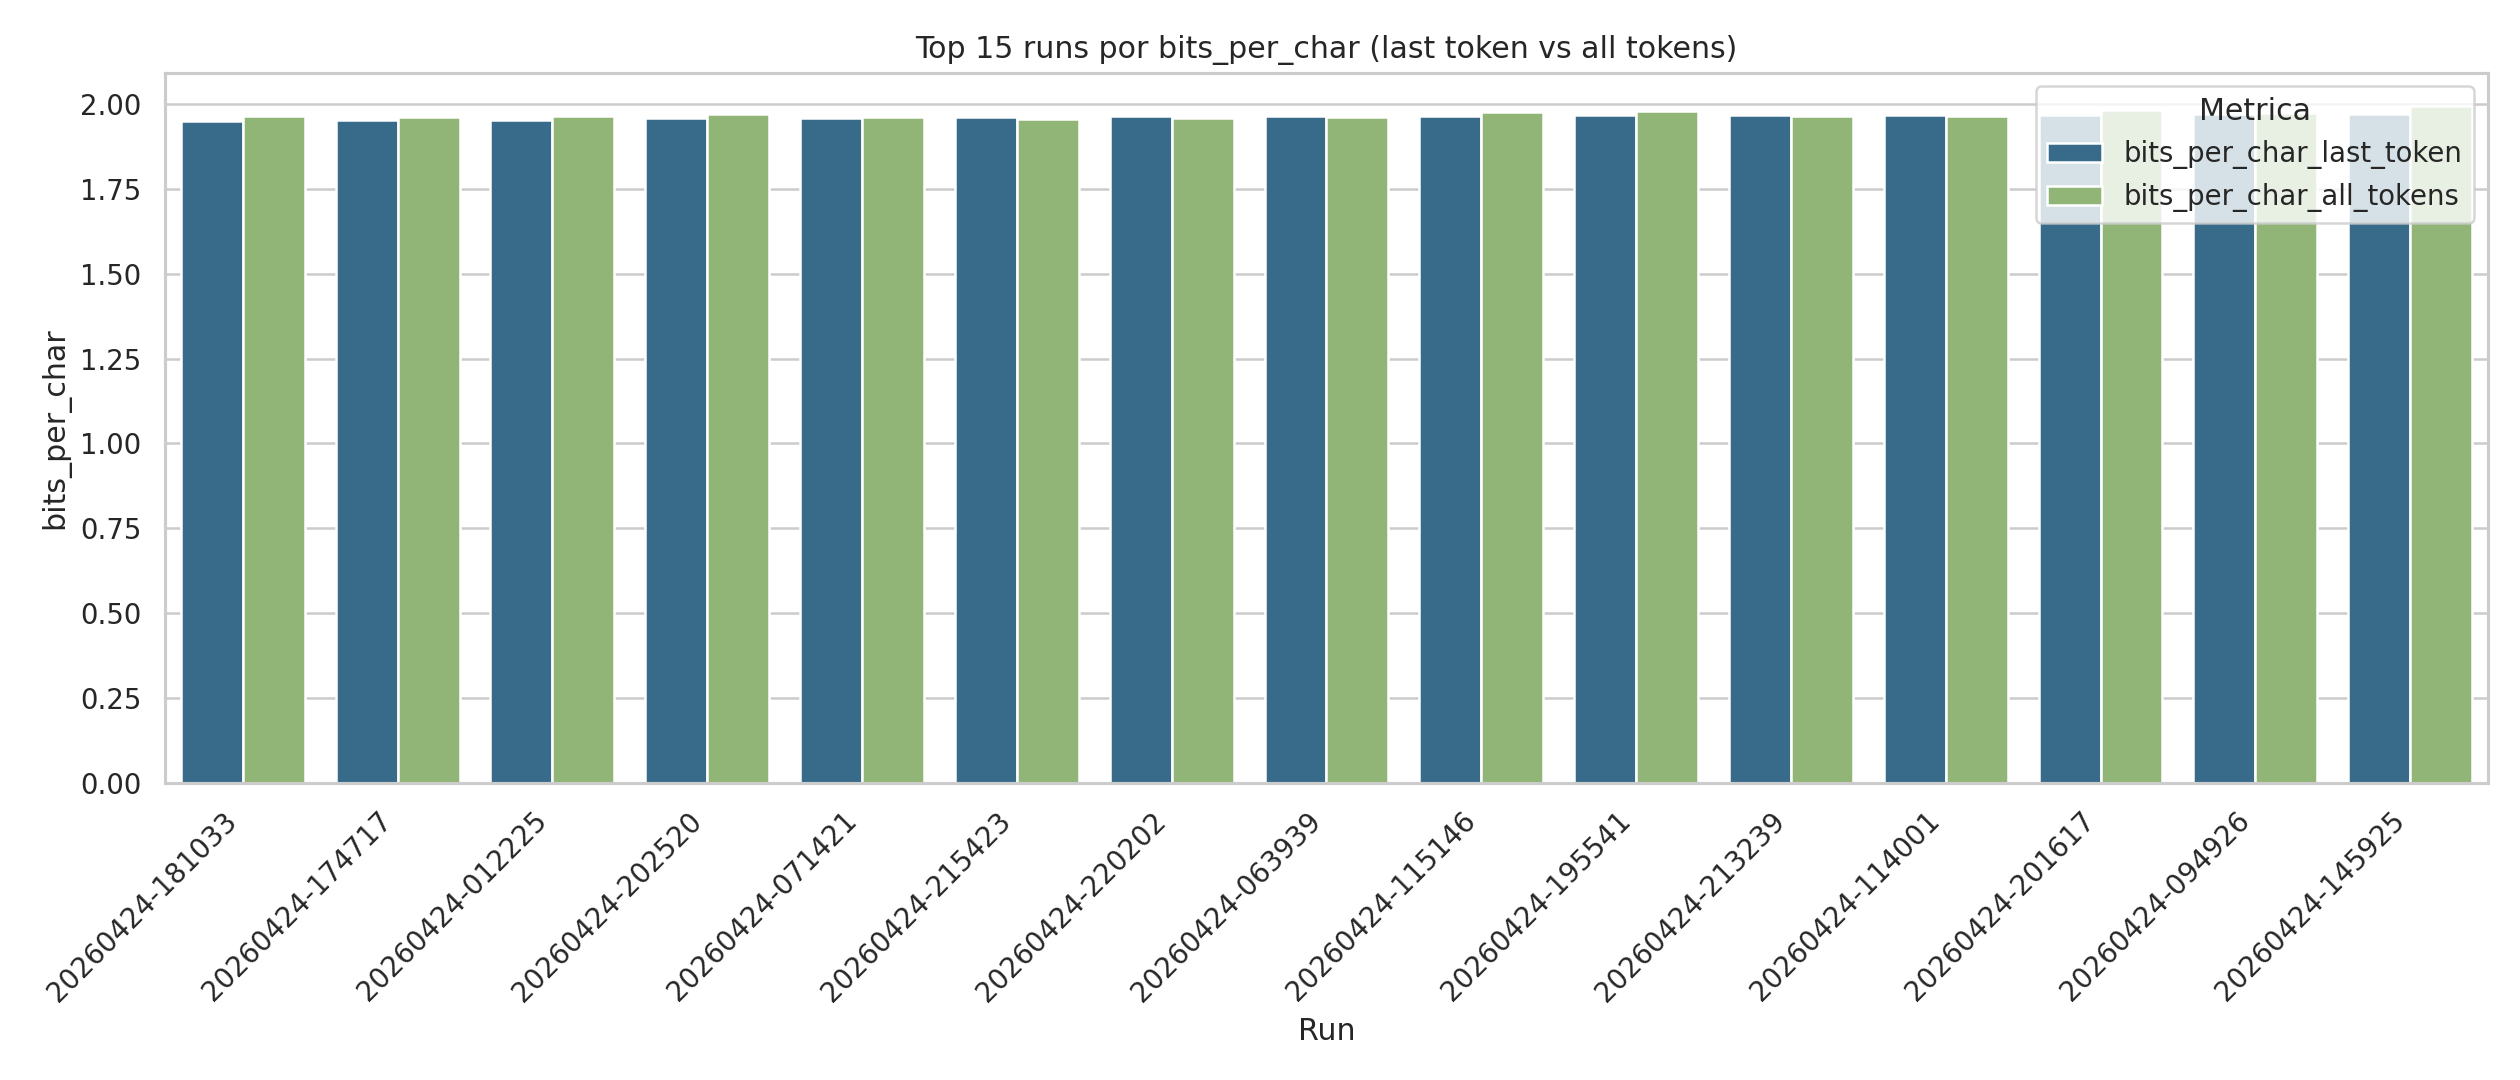
\includegraphics[width=0.85\textwidth]{../analysis/artifact_analysis/top_runs_dual_metrics.png}
    \caption{Comparación de los mejores experimentos del LLM con las dos métricas principales.}
\end{figure}

La comparación de los mejores experimentos muestra que no siempre coincide el mejor modelo según \texttt{bpc\_all\_tokens} y según \texttt{bpc\_last\_token}. Por ello, no se seleccionó únicamente el mínimo absoluto de una métrica, sino una configuración equilibrada entre ambas. El modelo elegido mantiene un rendimiento muy competitivo cuando se evalúa el último token, pero sin empeorar de forma clara la métrica calculada sobre todas las posiciones.

\begin{figure}[H]
    \centering
    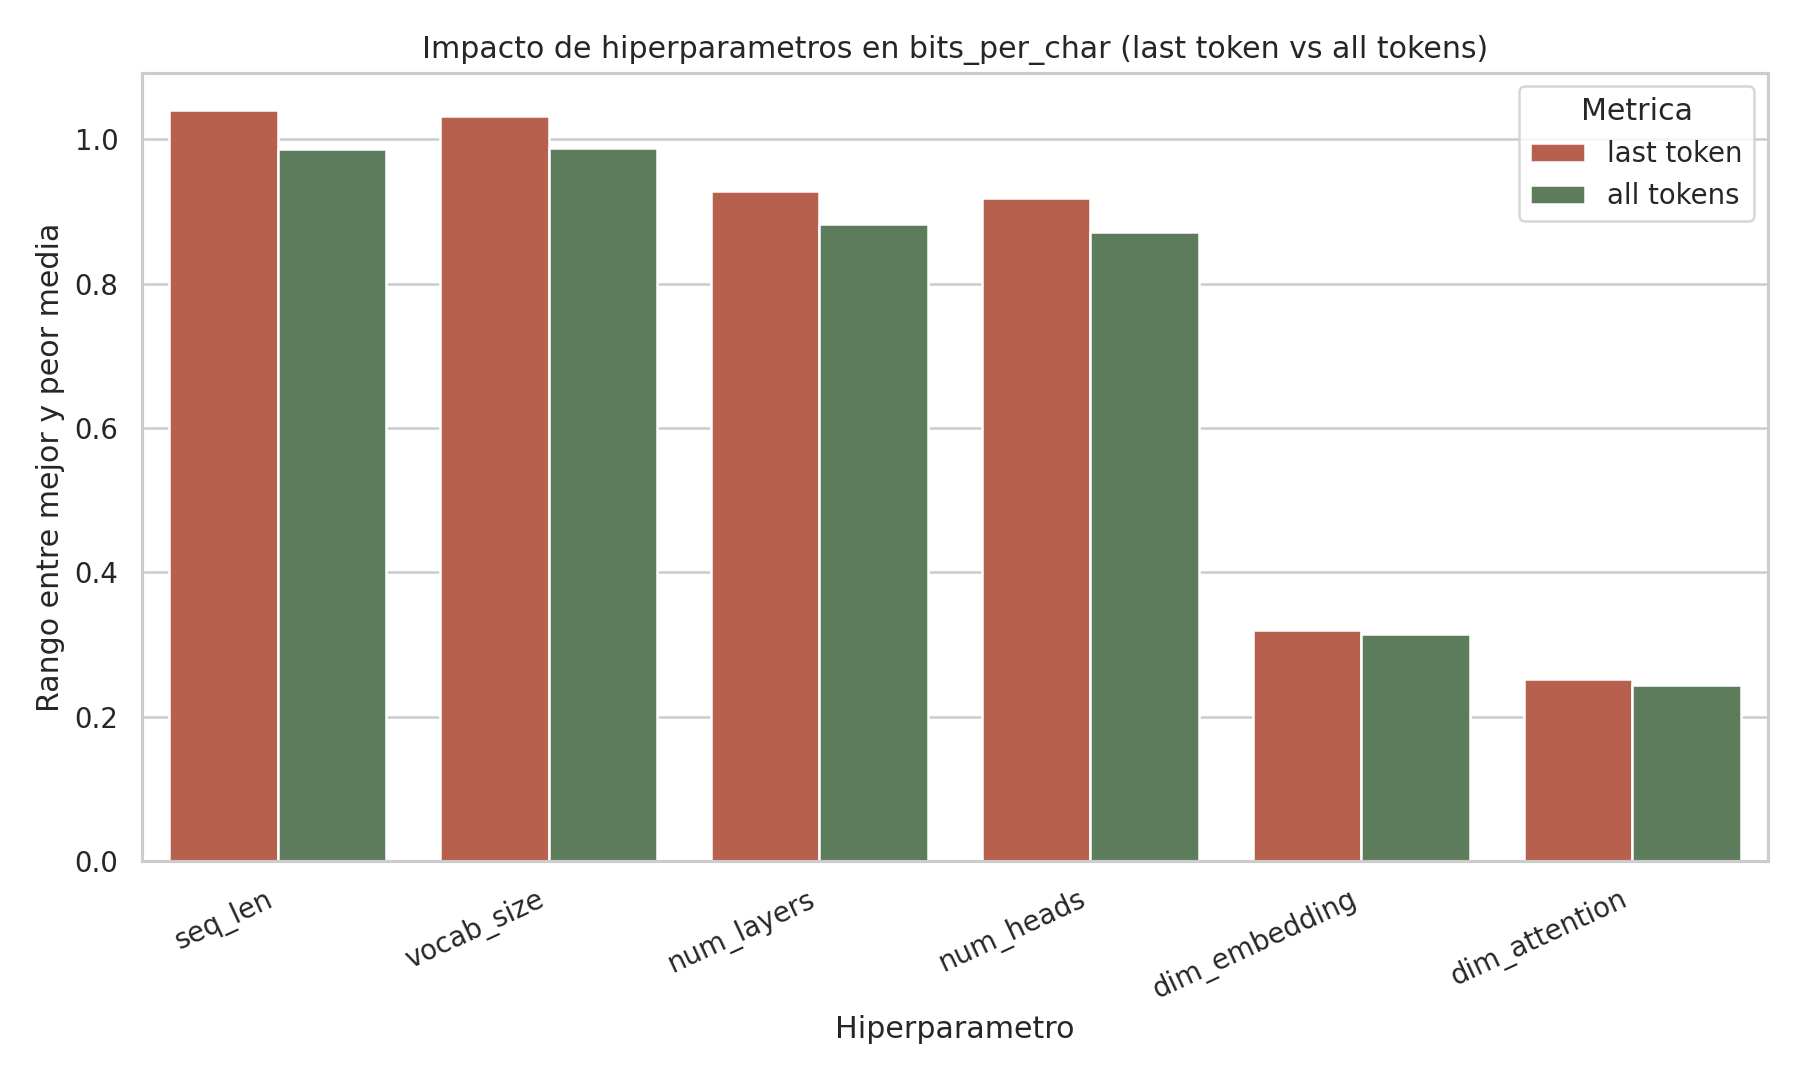
\includegraphics[width=0.85\textwidth]{../analysis/artifact_analysis/param_impact_dual_metrics.png}
    \caption{Impacto medio de los hiperparámetros sobre el rendimiento.}
\end{figure}

El análisis agregado por hiperparámetro indica que las variables con mayor impacto medio fueron \texttt{seq\_len} y \texttt{vocab\_size}. Esto es coherente con el problema: el tamaño del vocabulario modifica la granularidad de la tokenización, mientras que la longitud de contexto determina cuánta información previa puede usar el modelo para predecir el siguiente token. El número de capas y de cabezas también influye, aunque en menor medida. Las dimensiones internas presentan un efecto menos marcado en la media global.

\begin{figure}[H]
    \centering
    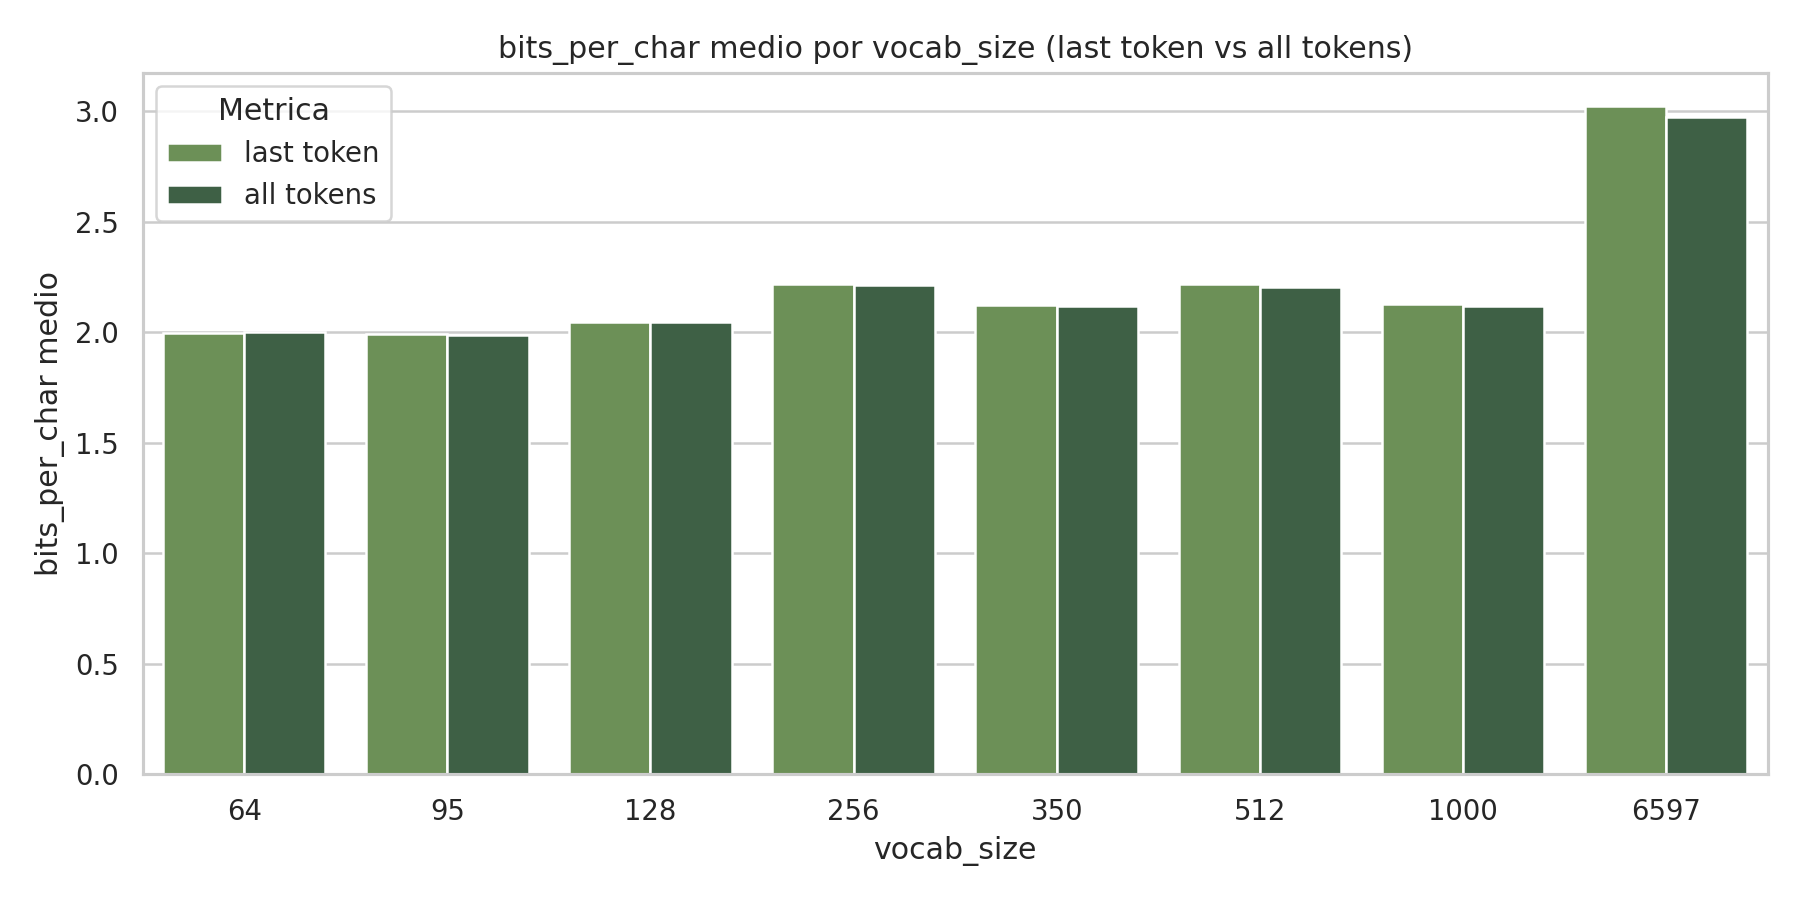
\includegraphics[width=0.8\textwidth]{../analysis/artifact_analysis/metric_by_vocab_size_dual_metrics.png}
    \caption{Bits por carácter medios en función de \texttt{vocab\_size}.}
\end{figure}

La gráfica por tamaño de vocabulario muestra que los mejores resultados se concentran en vocabularios pequeños o intermedios, especialmente alrededor de \texttt{vocab\_size=64} y \texttt{128}. En cambio, vocabularios demasiado grandes empeoran el rendimiento medio. Esto sugiere que, para el tamaño del corpus y del modelo utilizado, aumentar mucho el vocabulario no compensa: reduce la longitud de las secuencias, pero también incrementa el espacio de predicción y puede dificultar el aprendizaje.

\begin{figure}[H]
    \centering
    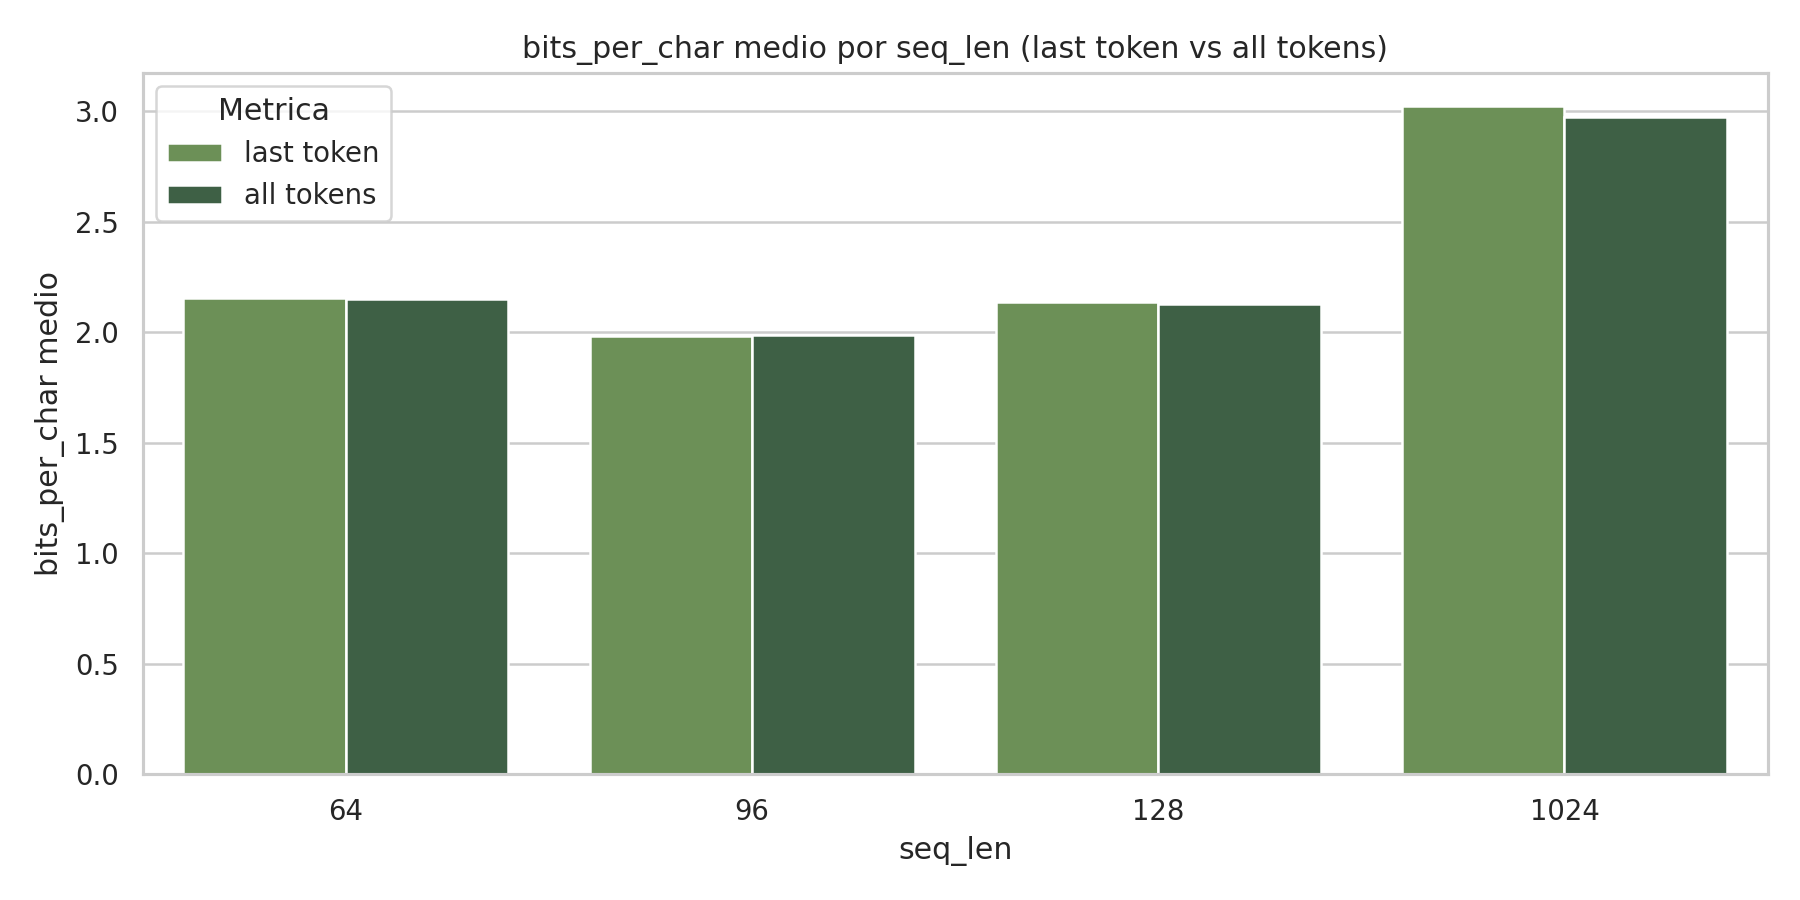
\includegraphics[width=0.8\textwidth]{../analysis/artifact_analysis/metric_by_seq_len_dual_metrics.png}
    \caption{Bits por carácter medios en función de \texttt{seq\_len}.}
\end{figure}

La longitud de contexto también tiene un efecto claro. Los mejores valores aparecen en longitudes moderadas, especialmente en torno a \texttt{seq\_len=96}. Longitudes demasiado pequeñas limitan el contexto disponible, mientras que longitudes muy grandes pueden introducir secuencias más difíciles de optimizar para un modelo pequeño y con pocos datos. Por tanto, la mejor zona se encuentra en un punto intermedio.

\begin{figure}[H]
    \centering
    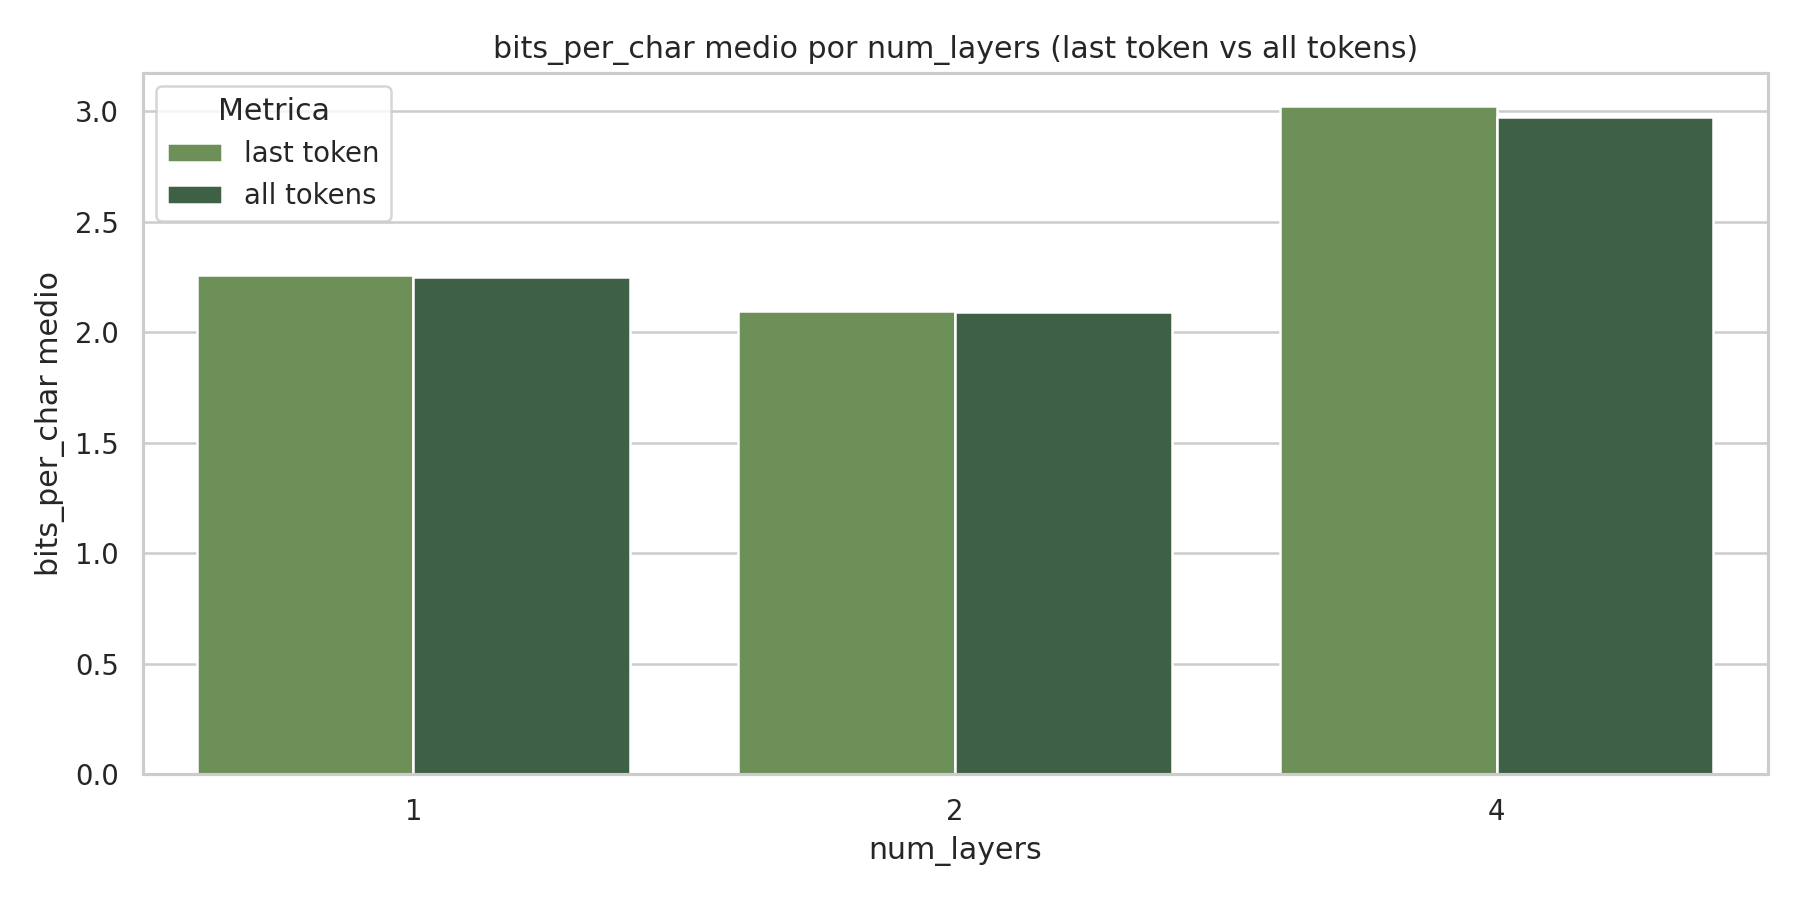
\includegraphics[width=0.8\textwidth]{../analysis/artifact_analysis/metric_by_num_layers_dual_metrics.png}
    \caption{Bits por carácter medios en función de \texttt{num\_layers}.}
\end{figure}

Respecto al número de capas, los mejores resultados se obtienen con arquitecturas poco profundas. En particular, las configuraciones con \texttt{num\_layers=2} aparecen de forma consistente entre los mejores experimentos. Aumentar la profundidad no mejoró el rendimiento medio, probablemente porque el tamaño del problema no justificaba modelos más complejos o porque estos eran más difíciles de entrenar de forma estable.

\begin{figure}[H]
    \centering
    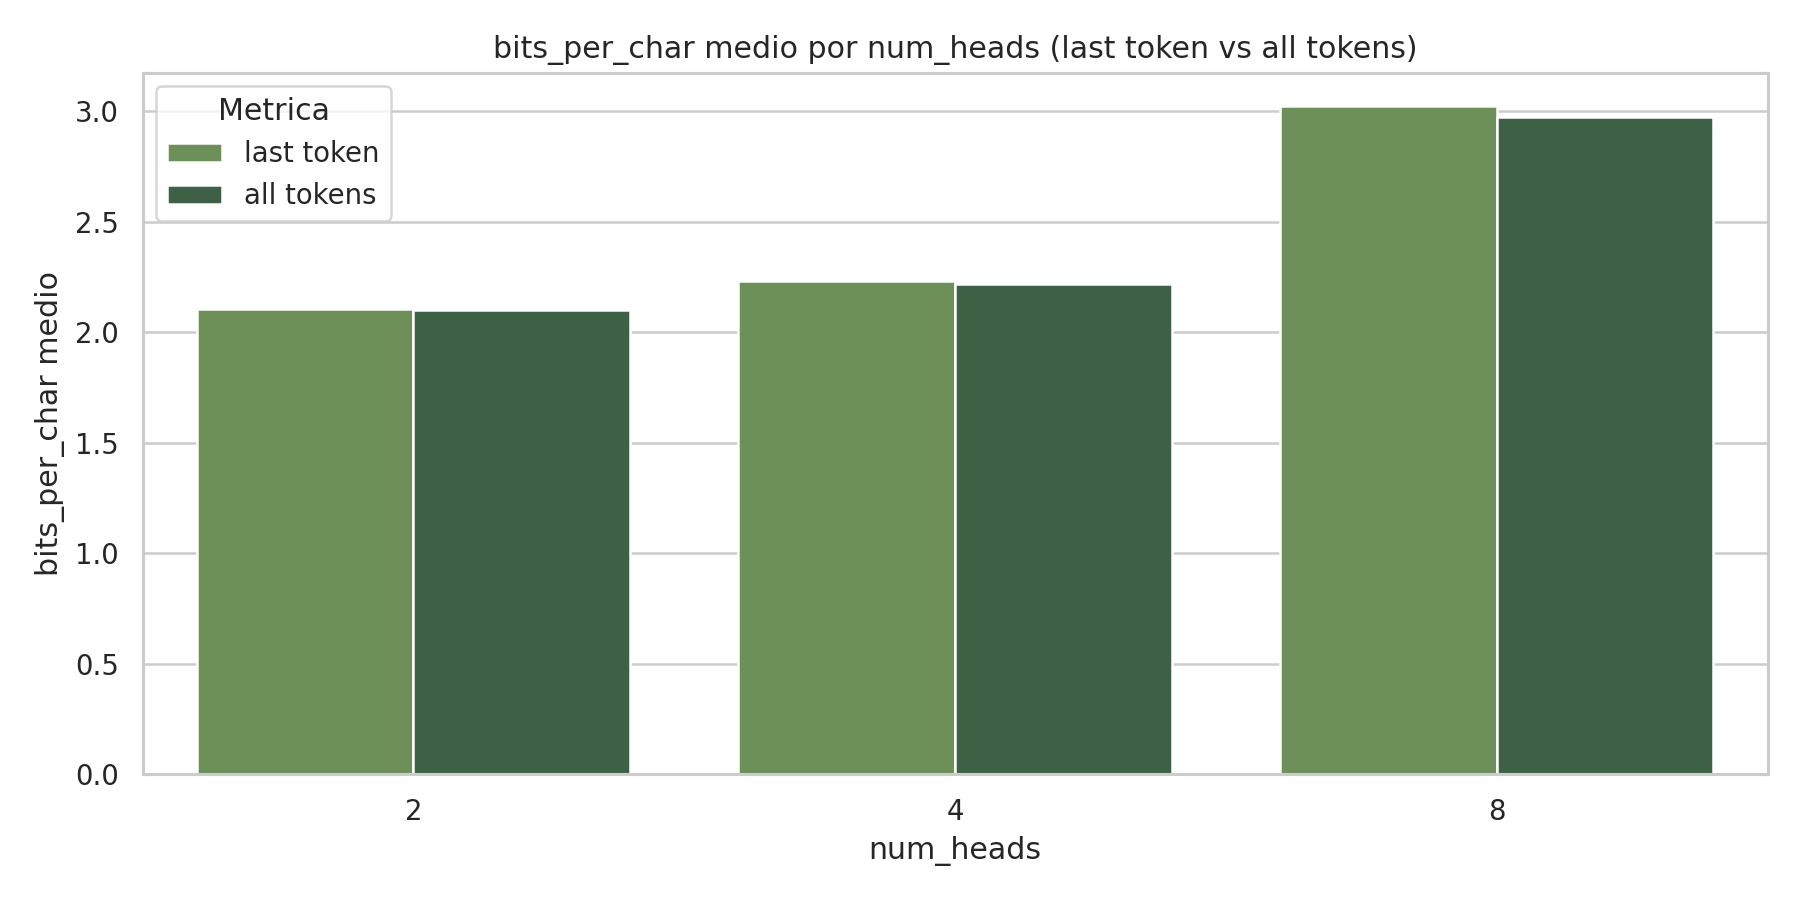
\includegraphics[width=0.8\textwidth]{../analysis/artifact_analysis/metric_by_num_heads_dual_metrics.png}
    \caption{Bits por carácter medios en función de \texttt{num\_heads}.}
\end{figure}

El comportamiento del número de cabezas sigue una tendencia similar. Las configuraciones con \texttt{num\_heads=2} resultan más competitivas que alternativas con más cabezas. Esto refuerza la idea de que, en este escenario, una arquitectura compacta aprovecha mejor los datos disponibles que un modelo más grande.

\begin{figure}[H]
    \centering
    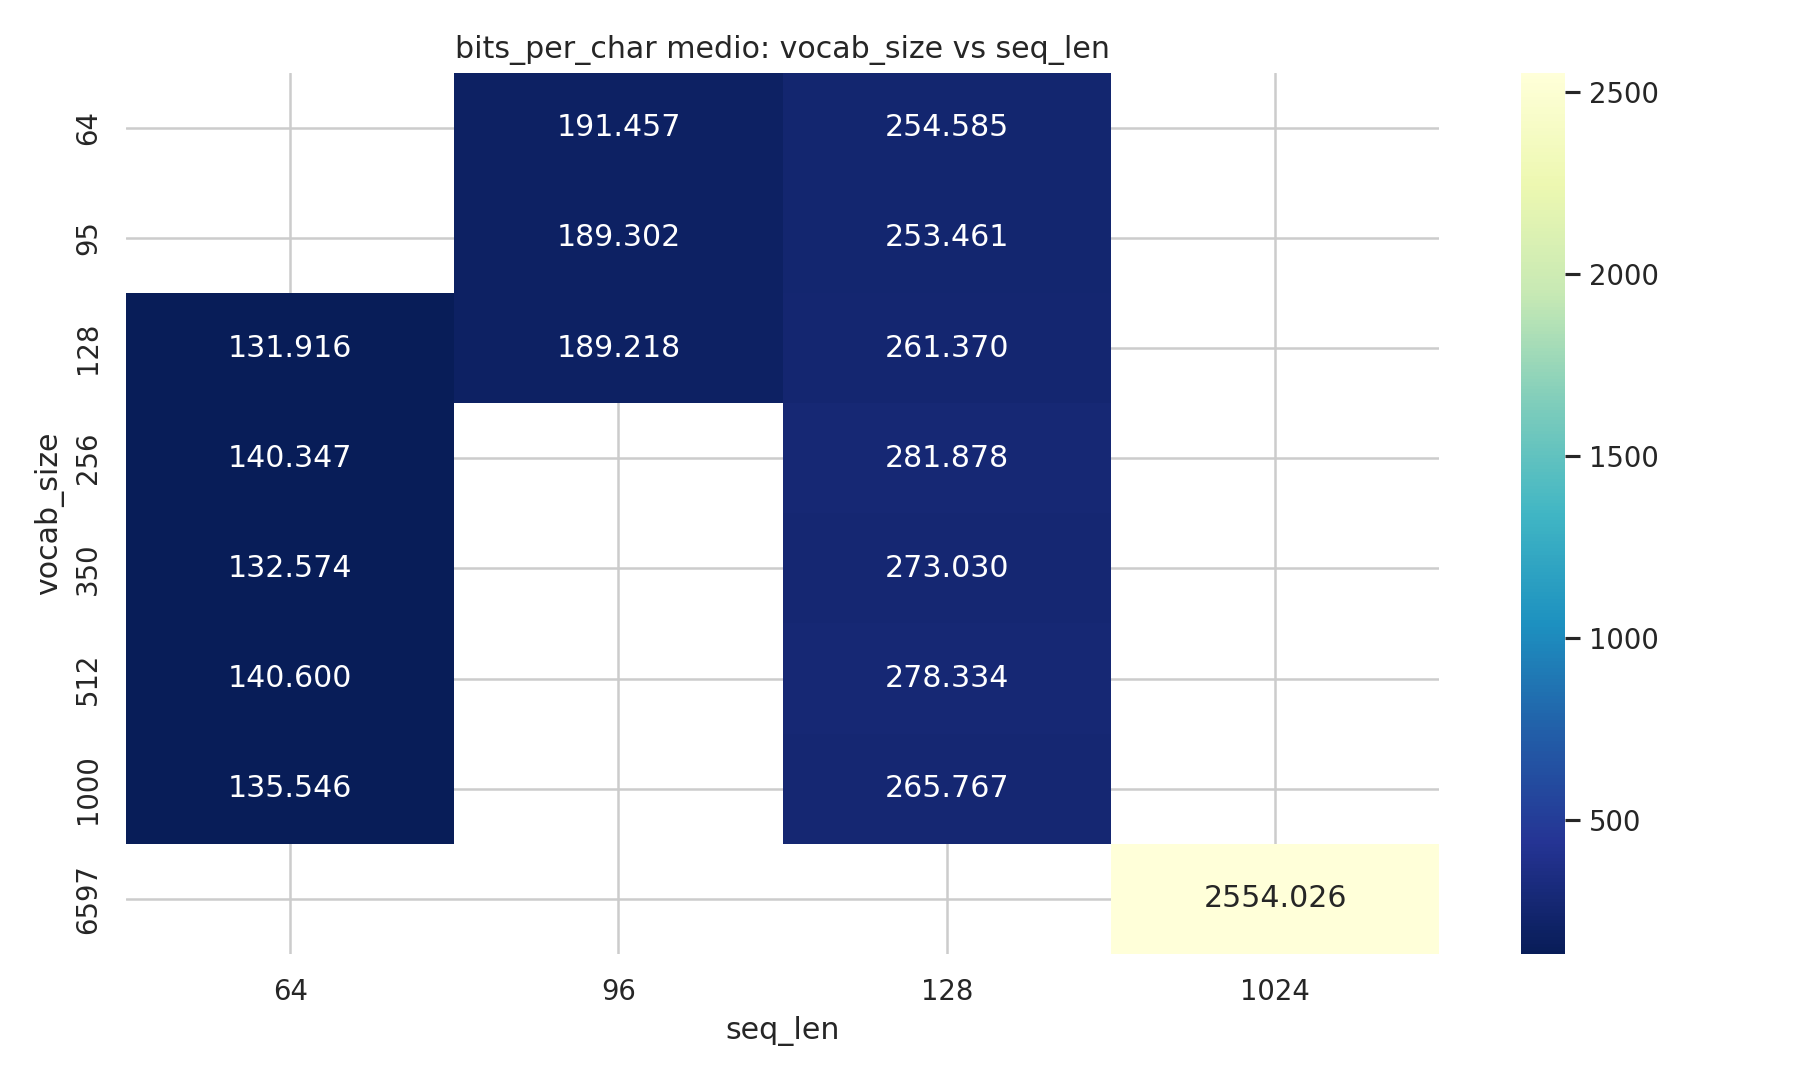
\includegraphics[width=0.8\textwidth]{../analysis/artifact_analysis/heatmap_vocab_seq_len.png}
    \caption{Interacción entre \texttt{vocab\_size} y \texttt{seq\_len} sobre el rendimiento medio.}
\end{figure}

Por último, el mapa de calor entre \texttt{vocab\_size} y \texttt{seq\_len} muestra que ambos hiperparámetros deben interpretarse conjuntamente. El tamaño del vocabulario afecta a cuántos tokens se generan para representar un texto, y la longitud de contexto fija cuántos de esos tokens puede observar el modelo. La mejor región se concentra en vocabularios pequeños o medios y longitudes de contexto moderadas, lo que coincide con la configuración final seleccionada.

En conjunto, los resultados del LLM indican que las configuraciones más grandes no fueron necesariamente mejores. La zona más competitiva del barrido corresponde a modelos compactos, con \texttt{vocab\_size} reducido o intermedio, \texttt{seq\_len} moderado, dos capas y dos cabezas de atención.

\section{Adaptación a NER}

Para la tarea de NER se reutilizó el mejor LLM como \textit{backbone} preentrenado. Sobre esta base se añadió una cabeza de clasificación para predecir la etiqueta de cada token y se realizó un nuevo barrido de hiperparámetros centrado en \texttt{batch\_size}, \texttt{epochs}, \texttt{learning\_rate} y \texttt{freeze\_backbone}.

En esta segunda fase se introdujeron dos cambios importantes respecto a la primera versión del sistema. En primer lugar, la función de pérdida pasó a ser una \textit{weighted cross entropy}, con pesos calculados a partir de la frecuencia de etiquetas en entrenamiento. El objetivo era reducir el sesgo hacia la clase \texttt{O}, muy dominante en el corpus, y dar más importancia a las etiquetas de entidades, mucho menos frecuentes. En segundo lugar, la selección del mejor modelo dejó de basarse en una métrica dominada por la clase mayoritaria y pasó a usar \texttt{val\_entity\_token\_f1\_micro}, calculada únicamente sobre las etiquetas de entidad y utilizada tanto para escoger el mejor checkpoint de cada entrenamiento como para actualizar el mejor artefacto global en \texttt{artifacts/ner/best}.

La mejor configuración encontrada fue:

\begin{itemize}
    \item \texttt{freeze\_backbone=False}
    \item \texttt{learning\_rate=1e-3}
    \item \texttt{batch\_size=8}
    \item \texttt{epochs=8}
    \item \texttt{best\_val\_entity\_token\_f1\_micro} $\approx$ \texttt{0.7169}
\end{itemize}

El mejor artefacto guardado en \texttt{artifacts/ner/best} corresponde a esta configuración. En el grid search apareció también una variante con \texttt{epochs=12} que alcanzó exactamente el mismo máximo de \texttt{val\_entity\_token\_f1\_micro}, pero sin superar el mejor valor ya registrado. Por tanto, se conservó la versión de 8 épocas como mejor candidato global. El resultado más importante es que el mejor rendimiento se obtuvo realizando \textit{fine-tuning} completo, es decir, actualizando también los pesos del \textit{backbone}. Esto indica que las representaciones aprendidas durante el entrenamiento del LLM son útiles como punto de partida, pero todavía necesitan adaptarse a la tarea específica de etiquetado secuencial.

\begin{figure}[H]
    \centering
    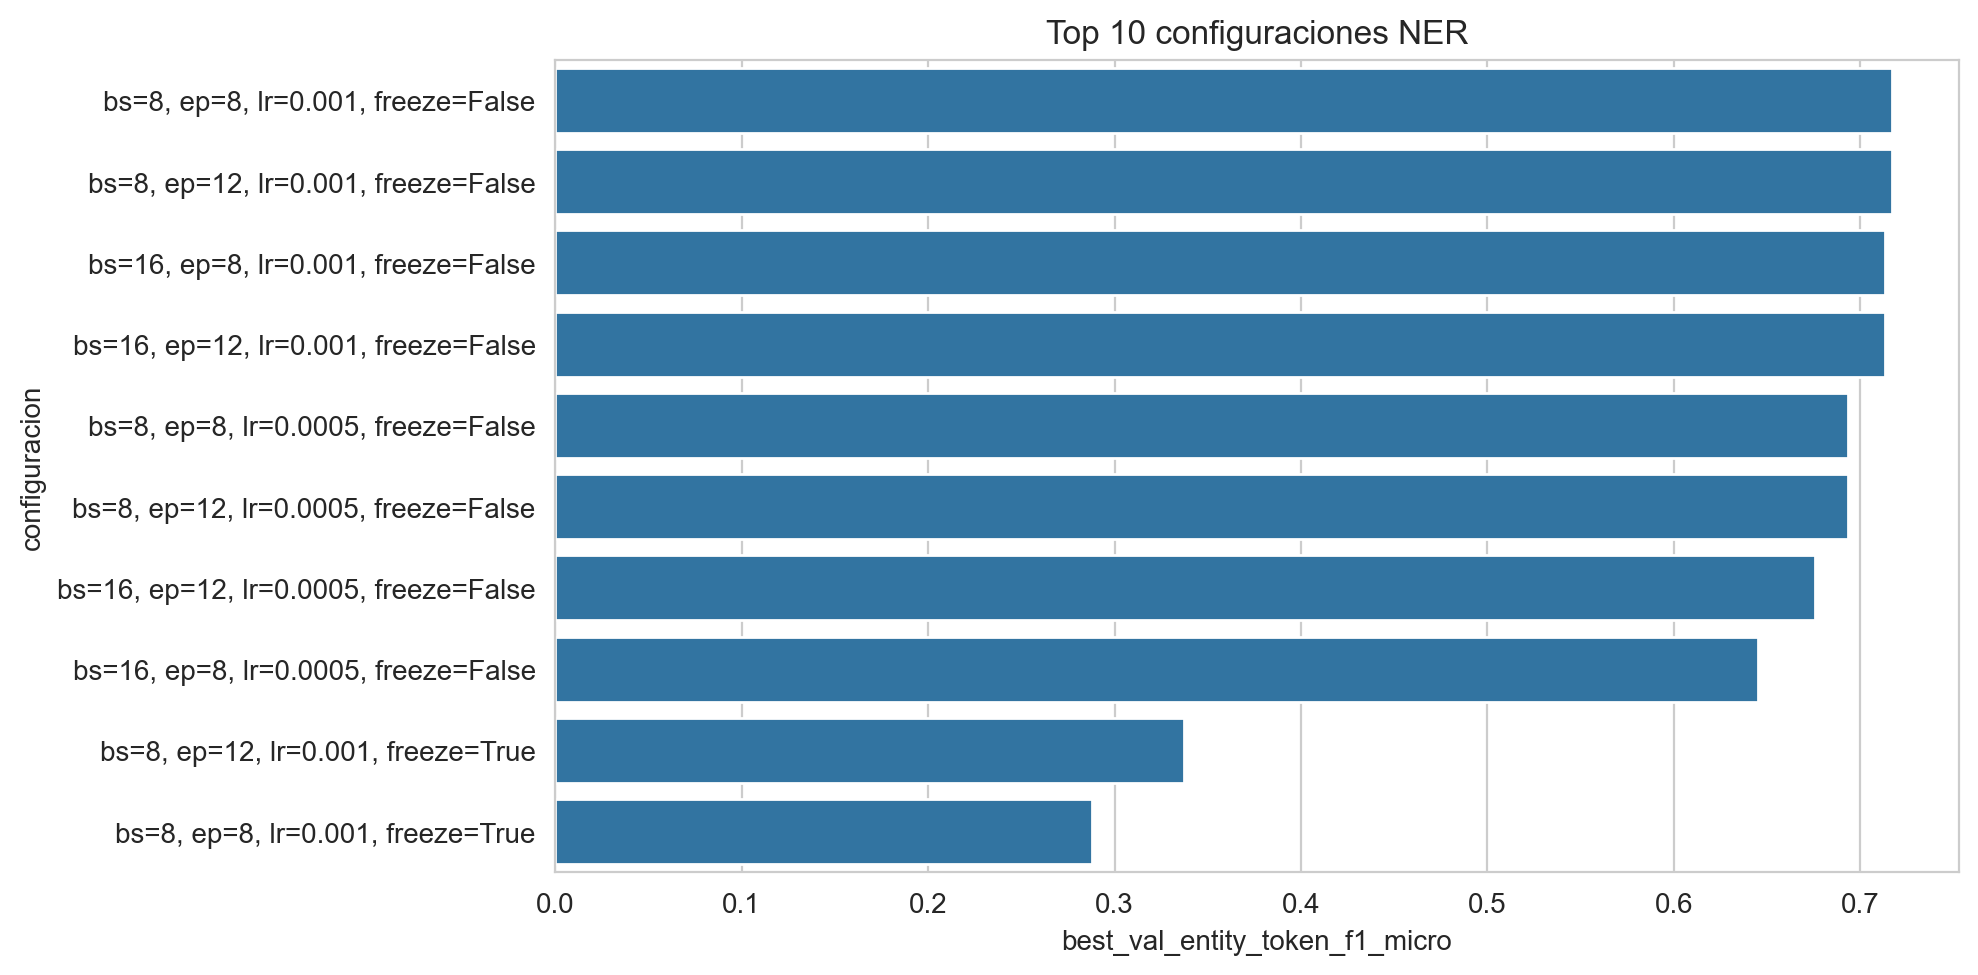
\includegraphics[width=0.85\textwidth]{../analysis/artifact_ner_analysis/top10_ner_configs.png}
    \caption{Mejores configuraciones evaluadas para NER.}
\end{figure}

\begin{figure}[H]
    \centering
    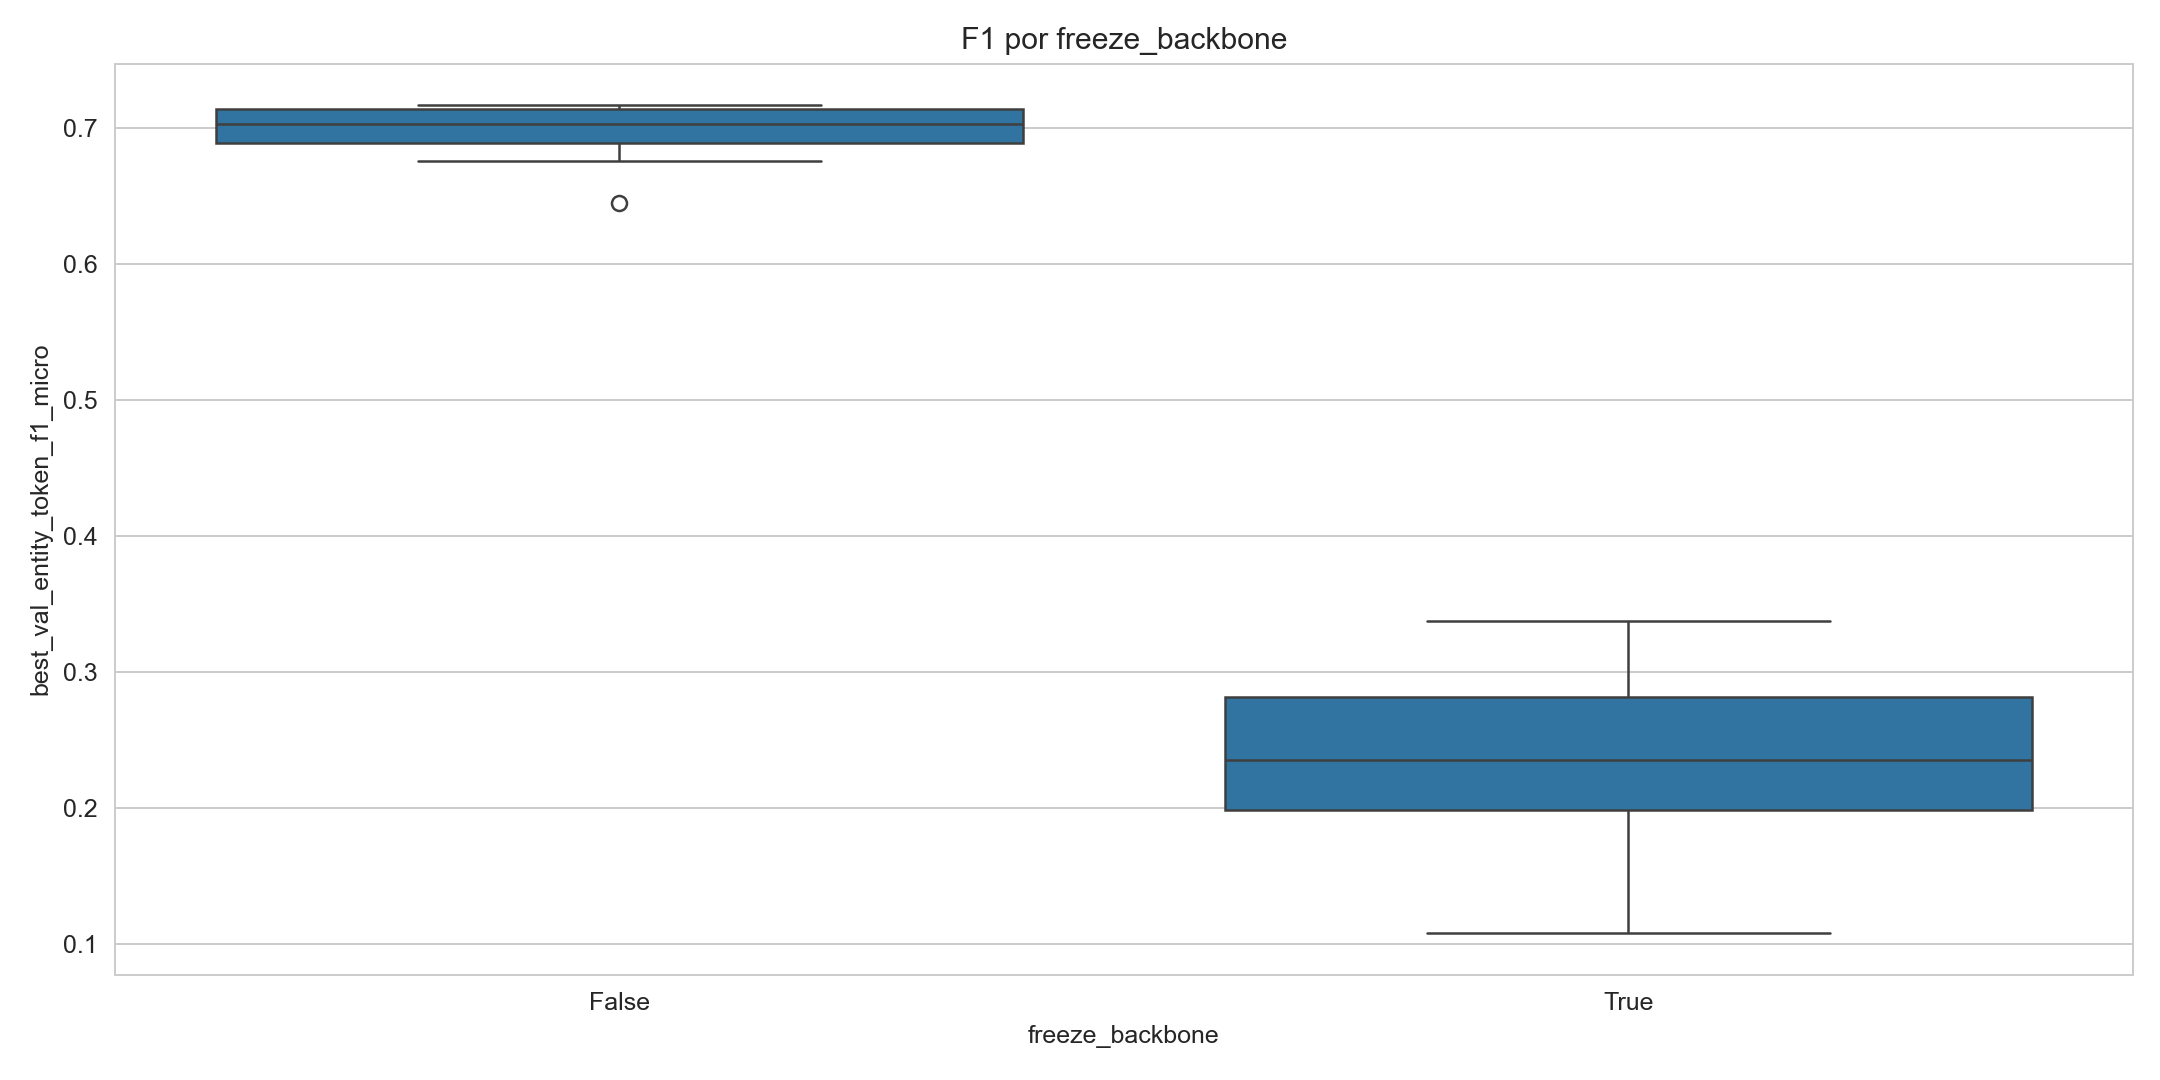
\includegraphics[width=0.7\textwidth]{../analysis/artifact_ner_analysis/f1_by_freeze_backbone.png}
    \caption{Distribución de \texttt{val\_entity\_token\_f1\_micro} según \texttt{freeze\_backbone}.}
\end{figure}

La comparación de las mejores configuraciones muestra que los experimentos más competitivos aparecen principalmente cuando \texttt{freeze\_backbone=False}. En cambio, congelar el \textit{backbone} limita la capacidad del modelo para ajustar sus representaciones internas a las entidades del conjunto NER. Con la nueva métrica centrada en entidades esta diferencia se vuelve especialmente clara: los modelos congelados obtienen accuracies razonables por el predominio de \texttt{O}, pero quedan muy por debajo cuando se evalúa solo la capacidad real de recuperar entidades. Por tanto, aunque el preentrenamiento proporciona una inicialización útil, la adaptación completa del modelo resulta clave para alcanzar el mejor rendimiento sobre entidades.

\begin{figure}[H]
    \centering
    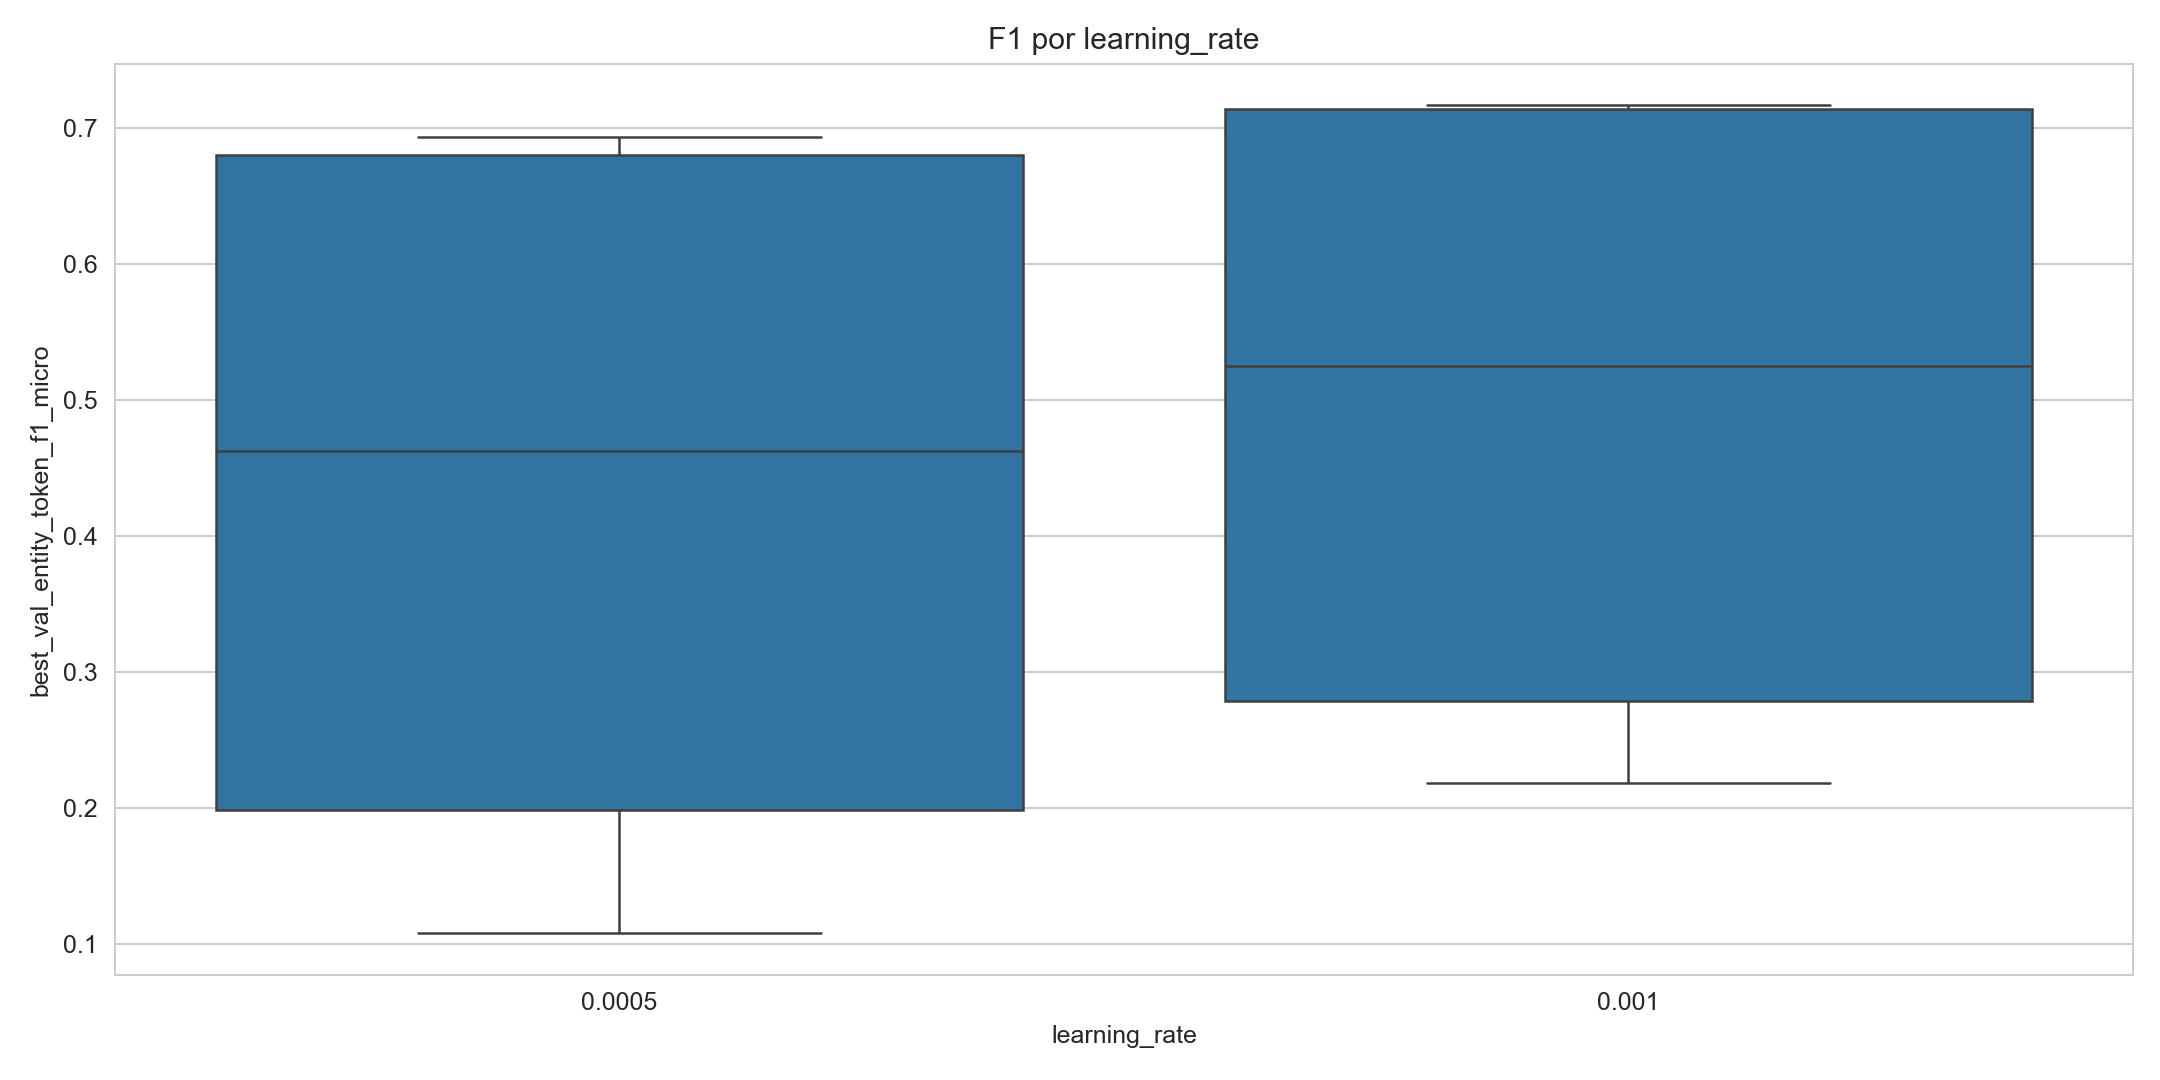
\includegraphics[width=0.75\textwidth]{../analysis/artifact_ner_analysis/f1_by_learning_rate.png}
    \caption{Distribución de \texttt{val\_entity\_token\_f1\_micro} en función del \textit{learning rate}.}
\end{figure}

La gráfica por \textit{learning rate} indica que \texttt{1e-3} fue el valor más efectivo. Los valores menores tienden a producir resultados ligeramente peores, probablemente porque el ajuste del modelo avanza de forma más lenta y no aprovecha completamente las épocas disponibles. En este caso, \texttt{1e-3} parece ofrecer un buen equilibrio entre velocidad de adaptación y estabilidad del entrenamiento.

\begin{figure}[H]
    \centering
    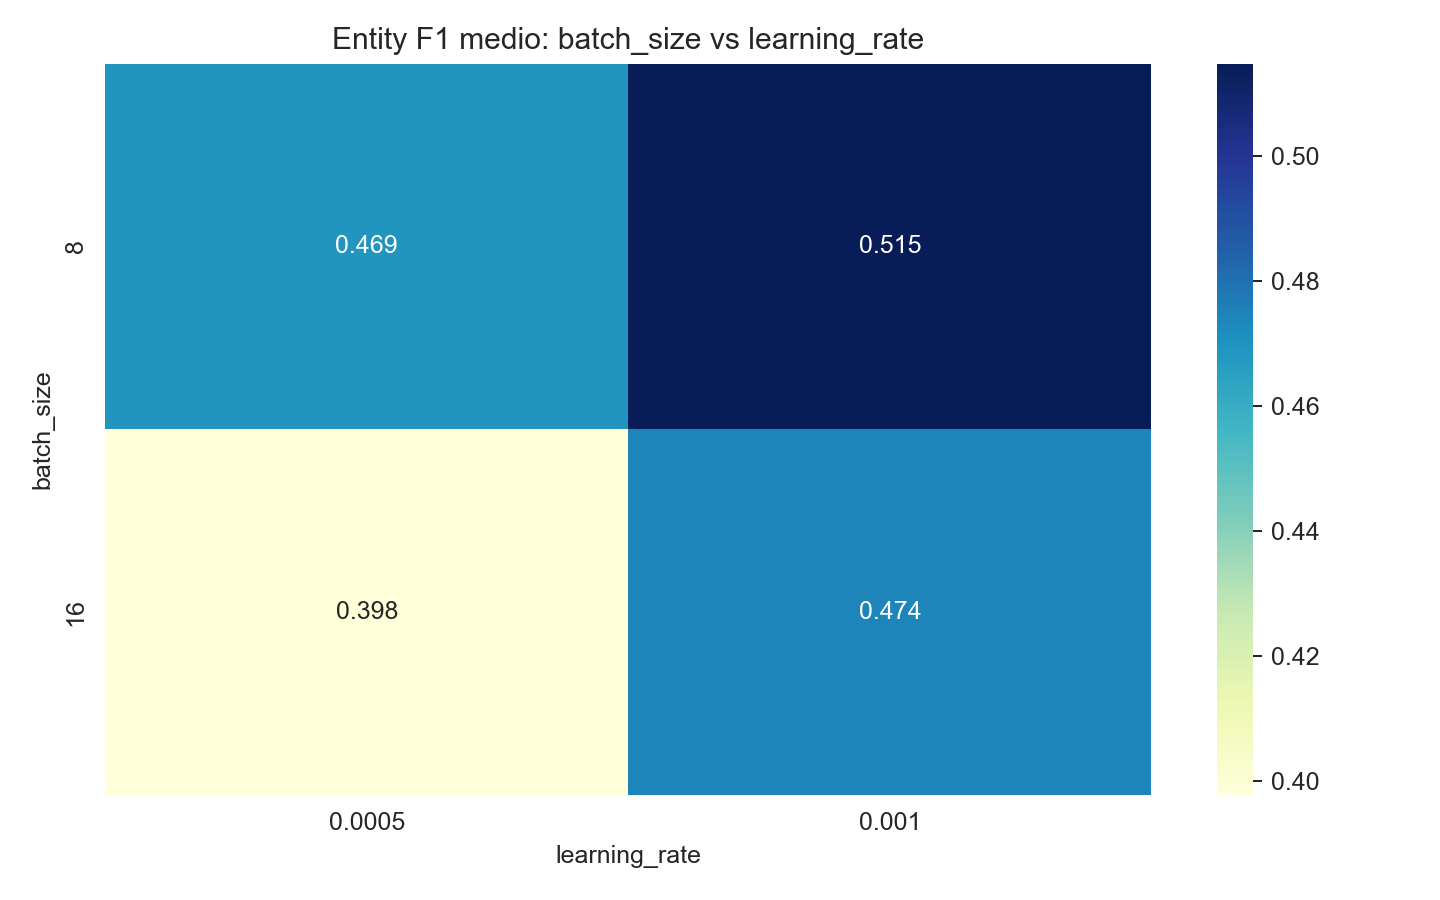
\includegraphics[width=0.75\textwidth]{../analysis/artifact_ner_analysis/heatmap_batch_lr_f1.png}
    \caption{Relación entre \texttt{batch\_size}, \texttt{learning\_rate} y \texttt{val\_entity\_token\_f1\_micro}.}
\end{figure}

El mapa de calor entre \texttt{batch\_size} y \texttt{learning\_rate} muestra que la mejor región aparece en la combinación de \texttt{learning\_rate=1e-3} con \texttt{batch\_size} pequeño. En concreto, \texttt{batch\_size=8} produjo el mejor valor de la métrica principal, mientras que \texttt{batch\_size=16} quedó ligeramente por debajo. Además, aumentar el número de épocas de 8 a 12 no mejoró el máximo alcanzado, lo que sugiere que el modelo llega pronto a su mejor zona y que entrenar más no aporta una ventaja clara en este escenario.

En conjunto, los resultados de NER muestran que el modelo preentrenado no debe utilizarse únicamente como extractor fijo de características. El mejor comportamiento se consigue permitiendo que todo el modelo se adapte a la nueva tarea, utilizando una pérdida ponderada para compensar el desbalanceo de clases y evaluando el sistema con una métrica centrada en entidades en lugar de depender solo de la accuracy o de una métrica dominada por la clase \texttt{O}.

\section{Conclusiones}

El barrido del LLM muestra que, al comparar modelos con tokenizadores distintos, es preferible usar métricas normalizadas por carácter en lugar de depender solo de la pérdida por token. La clave es transformar la pérdida a escala de carácter antes de expresarla en bits, ya que esto permite comparar modelos con distinto \texttt{vocab\_size} sobre una unidad común.

La mejor configuración del LLM corresponde a un modelo compacto, con vocabulario pequeño, longitud de contexto moderada y una arquitectura de dos capas y dos cabezas. Los resultados indican que, para este escenario, aumentar el tamaño del modelo no aporta necesariamente una mejora y puede empeorar la optimización.

En la tarea de NER, el mejor resultado se obtuvo reutilizando el LLM preentrenado y realizando \textit{fine-tuning} completo. Congelar el \textit{backbone} dio peores resultados, lo que confirma que las representaciones aprendidas por el LLM son útiles, pero deben adaptarse a la tarea final. La configuración más estable combinó \texttt{learning\_rate=1e-3}, \texttt{batch\_size=8} y \texttt{8} épocas, alcanzando una \texttt{best\_val\_entity\_token\_f1\_micro} aproximada de \texttt{0.7169}. El uso de pérdida ponderada y de una métrica centrada en entidades permitió evaluar de forma más fiel el rendimiento real del sistema bajo fuerte desbalanceo de clases.

En conjunto, los experimentos muestran que un LLM pequeño, correctamente evaluado y ajustado, puede servir como base eficaz para una tarea posterior de etiquetado secuencial como NER.

\end{document}
